\documentclass{article}
\usepackage[utf8]{inputenc}
\usepackage[margin=1in]{geometry}
\usepackage[fleqn]{amsmath}
\usepackage{tikz-qtree}
\usepackage{multirow}

\title{Problem Set 2}
\author{Edith Zeng (xz4842)\\Intro to Machine Learning\\Dr. Danna Gurari, Fall 2018}

\begin{document}

\maketitle

\section{Decision Tree}
\subsection{(a)}
For the binary value of ``Satisfied", $C_1 = Yes$, $C_2 = No.$
\\
The current entropy can be calculated as 
\[ \boldsymbol{Entropy} = - \sum_{i=1}^2Pr(i)\log_{2}Pr(i) \] \[
= -P(Satisfied=``Yes")\log_{2}P(Satisfied=``Yes") \]\[- P(Satisfied=``No")\log_{2}\,P(Satisfied=``No")
\]
\[
= -\frac{5}{8}\times \log_{2}\frac{5}{8}-\frac{3}{8}\times \log_{2}\frac{3}{8} 
\]
\[\approx 0.9544
\]

\begin{itemize}
    \item If we split on the feature \textbf{``Clean"}, the left tree is ``Yes" and the right tree is ``No". The entropy on this level can be calculated as:
    \[\boldsymbol{Entropy_{\,left}} = - P(Satisfied=``Yes"|Clean=``Yes")\,\log_{2}P(Satisfied=``Yes"|Clean=``Yes") \]\[ -P(Satisfied=``No"|Clean=``Yes")\,\log_{2}P(Satisfied=``No"|Clean=``Yes")\]
    \[= -\frac{2}{4}\times \log_{2}\frac{2}{4} - \frac{2}{4}\times \log_{2}\frac{2}{4} = 1\]
    
    \[\boldsymbol{Entropy_{\,right}} = -P(Satisfied=``Yes"|Clean=``No")\,\log_{2}P(Satisfied=``Yes"|Clean=``No") \]\[ P(Satisfied=``No"|Clean=``No")\,\log_{2}P(Satisfied=``No"|Clean=``No")\]
    \[
    = -\frac{3}{4}\times \log_{2}\frac{3}{4} - \frac{1}{4}\times \log_{2}\frac{1}{4}\approx 0.8113
    \]
    
    The information gain is
    \[ \boldsymbol{IG_{split\,on\,``Clean"}} = Entropy - (\frac{4}{8}\times Entropy_{\,left}+\frac{4}{8}\times Entropy_{\,Right}) \]\[= 0.9544 - (\frac{1}{2}\times1+\frac{1}{2}\times0.8113) \approx 0.049\]
    
    \item If we split on \textbf{``Rent"}, there are several ways to split the tree.\\
    (1) Left Tree: rent $< 800$; right tree: rent $\geq 800$.
        \[
        \boldsymbol{Entropy_{\,left}} = -P(Satisfied=``Yes"|Rent<800)\log_{2}P(Satisfied=``Yes"|Rent<800)\]\[ -P(Satisfied=``No"|Rent<800)\log_{2}P(Satisfied=``No"|Rent<800)\]\[ = -\frac{4}{5}\times \log_{2}\frac{4}{5}-\frac{1}{5}\times \log_{2}\frac{1}{5}\approx 0.7219
        \]
        \[\boldsymbol{Entropy_{\,right}} =
        -P(Satisfied=``Yes"|Rent\geq 800)\log_{2}P(Satisfied=``Yes"|Rent\geq 800) \]\[- 
        P(Satisfied=``No"|Rent\geq 800)\log_{2}P(Satisfied=``No"|Rent\geq 800)
        \]\[ = -\frac{1}{3}\times\log_2\frac{1}{3}-\frac{2}{3}\times\log_2\frac{2}{3} \approx 0.9183\]
        The Information gain is
        \[\boldsymbol{IG_{split\,on``Rent"\,at\,800}} = Entropy - (\frac{5}{8}\times Entropy_{\,left} + \frac{3}{8}\times Entropy_{\,right})\]\[ 0.9544-(\frac{5}{8}\times0.7219+\frac{3}{8}\times0.9183)\approx0.159\]
    (2) Left tree: rent $< 700$; right tree: rent $\geq 700$.
    \[\boldsymbol{Entropy_{\,left}} = -P(Satisfied=``Yes"|Rent < 700)\log_2P(Satisfied=``Yes"|Rent < 700)\]\[-P(Satisfied=``No"|Rent < 700)\log_2P(Satisfied=``No"|Rent < 700)\]\[= -\frac{4}{4}\times\log_2\frac{4}{4}-\frac{3}{4}\times\log_2\frac{3}{4} = 0 - \frac{3}{4}\times\log_2\frac{3}{4}\approx0.3113\]
    \[\boldsymbol{Entropy_{\,right}} = -P(Satisfied=``Yes"|Rent\geq700)\log_2P(Satisfied=``Yes"|Rent\geq700) \]\[ -P(Satisfied=``No"|Rent\geq700)\log_2P(Satisfied=``No"|Rent\geq700)\]\[ =-\frac{1}{4}\times\log_2\frac{1}{4}-\frac{3}{4}\times\log_2\frac{3}{4} \approx0.8113 \]
    The information gain is
    \[ \boldsymbol{IG_{split\,on``rent"\,at\,700}} = Entropy - (\frac{4}{8}\times Entropy_{\,left} + \frac{4}{8}\times Entropy_{\,right})\]\[
    = 0.9544 - (\frac{1}{2}\times0+\frac{1}{2}\times0.8113)\approx0.5488\]
    (3) Left tree: rent $\geq 1000$; right tree: rent $< 1000$. 
    \[
    \boldsymbol{{Entropy_{\,left}}} = -P(Satisfied=``Yes"|Rent\geq1000)\log_2P(Satisfied=``Yes"|Rent\geq1000)\]\[-P(Satisfied=``No"|Rent\geq1000)\log_2P(Satisfied=``No"|Rent\geq1000)
    \]\[ = -\frac{0}{2}\times\log_2\frac{0}{2}-\frac{2}{2}\times\log_2\frac{2}{2} = -log_2 1 = 0\]
    \[
    \boldsymbol{{Entropy_{\,right}}} = -P(Satisfied=``Yes"|Rent<1000)\log_2P(Satisfied=``Yes"|Rent<1000)\]\[-P(Satisfied=``No"|Rent<1000)\log_2P(Satisfied=``No"|Rent<1000)
    \]\[ = -\frac{5}{6}\log_2\frac{5}{6} - \frac{1}{6}\log_2\frac{1}{6} \approx 0.6500\]
    The information gain is 
    \[\boldsymbol{IG_{split\,on``rent"\,at\,1,000}} = Entropy - (\frac{2}{8}\times Entropy_{left} + \frac{6}{8}\times Entropy_{right}) \]\[ = 0.9544 - (\frac{1}{4}\times0 + \frac{3}{4}\times0.6500)\approx0.467 \]
    (4) Left tree: rent $\leq 500$; right tree: rent $> 500$
    \[
    \boldsymbol{Entropy_{\,left}} = -P(Satisfied=``Yes"|rent\leq500)\log_2P(Satisfied=``Yes"|rent\leq500)\]\[-P(Satisfied=``No"|rent\leq500)log_2P(Satisfied=``No"|rent\leq500)\]\[= -\frac{2}{2}\log_2\frac{2}{2} - \frac{0}{2}\log_2\frac{0}{2} = 0
    \]
    \[
    \boldsymbol{Entropy_{\,right}} = -P(Satisfied=``Yes"|rent>500)\log_2P(Satisfied=``Yes"|rent>500)\]\[-P(Satisfied=``No"|rent>500)log_2P(Satisfied=``No"|rent>500)\]\[= -\frac{3}{6}\log_2\frac{3}{6} - \frac{3}{6}\log_2\frac{3}{6} = 1
    \]
    The information gain is 
    \[\boldsymbol{IG_{split\,on``rent"at\,500}} = Entropy - (\frac{2}{8}\times Entropy_{left} + \frac{6}{8}\times Entropy_{right})\]\[=0.9544 - (\frac{1}{4}\times0+\frac{3}{4}\times1)\approx0.204\]

    \item Based on the information gain scores above, the optimal feature to start splitting is Rent = 700. Repeat until entropy is zero. The decision tree looks like the following:
\\ \\
\tikzset{every tree node/.style={minimum width=2em,draw,circle},
         blank/.style={draw=none},
         edge from parent/.style=
         {draw,edge from parent path={(\tikzparentnode) -- (\tikzchildnode)}},
         level distance=1.5cm}
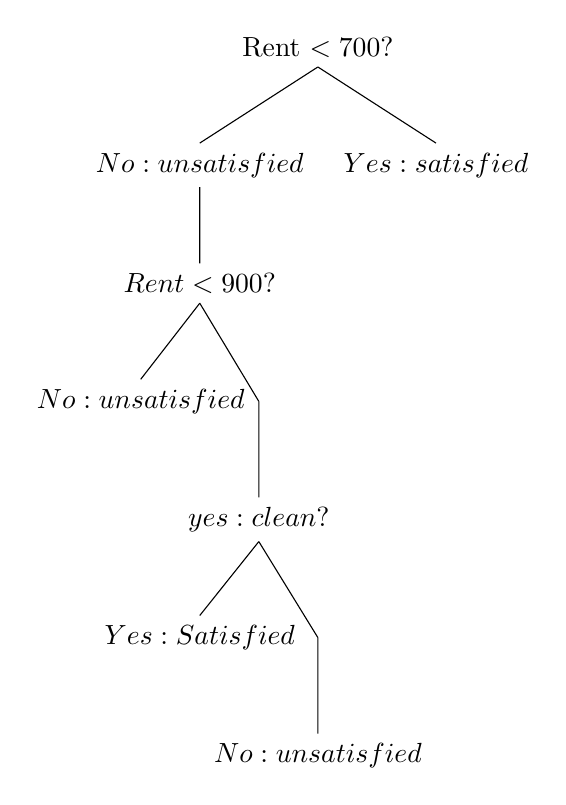
\begin{tikzpicture}[level distance=1.5cm,
  level 1/.style={sibling distance=3cm},
  level 2/.style={sibling distance=1.5cm}]
  \node {Rent $< 700?$}
    child {node {$No: unsatisfied$}
        child {
            node {$Rent < 900?$} {
                child {
                    node {$No:\\unsatisfied$}
                }
                child {
                    child{
                        node {$yes: clean?$} {
                            child {
                                node {$Yes: Satisfied\\$}
                            }
                            child {
                                child {
                                    node {$No:
                                    unsatisfied$}
                                    }
                        }
                    }
                    }
                }
            }
        }
    }
    child {
        node {$Yes: satisfied$}
    };
    
\end{tikzpicture}
\end{itemize}    

\subsection{(b)}
Prediction based on table 2:
\begin{table}[h]
\centering
\begin{tabular}{|c|c|c|c|c|}
\hline
Person & Rent (\$) & Satisfied? (actual) & Satisfied? (predicted) & test statistics \\ \hline
p9     & 1100      & No                  & No                     & TN              \\ \hline
p10    & 500       & Yes                 & Yes                    & TP              \\ \hline
p11    & 1300      & Yes                 & No                     & FN              \\ \hline
p12    & 550       & Yes                 & Yes                    & TP              \\ \hline
\end{tabular}
\caption{Decision tree classification results}
\end{table}

\subsection{(c)}
\[Precision = \frac{TP}{TP+FP} = \frac{2}{2+0} = 1\]
\[Recall = \frac{TP}{TP+FN} = \frac{2}{2+1} = \frac{2}{3}\]

\subsection{(d)}
\begin{table}[t]
\centering
\begin{tabular}{|c|c|c|c|}
\hline
                           & \multicolumn{3}{c|}{Actual} \\ \hline
\multirow{3}{*}{Predicted} &          & Yes     & No     \\ \cline{2-4} 
                           & Yes      & 2       & 0      \\ \cline{2-4} 
                           & No       & 1       & 1      \\ \hline
\end{tabular}
\caption{Confusion Matrix - Decision Tree}
\end{table}


\newpage

\section{Naive Bayes}
\subsection{(a)} 
Under the assumption of independence, the naive Bayes classifier models the posterior by calculating \[P(Satisfied=y_i|Rent=x) = \frac{P(Rent=x|Satisfied=y_i)\times P(Satisfied=y_i)}{\sum_{j=1}^{2}P(Rent=x|Satisfied=y_j)\times P(Satisfied=y_j)}\] where $y_i = \{``yes", ``no"\}$.

Assuming the data is drawn from a Gaussian distribution and share common variance across all classes, we can calculate class-specific means and variances using training data from Table 1:
\[ P(Satisfied=``Yes") = \frac{5}{8} \quad and\quad P(Satisfied=``No") = \frac{3}{8} \]
To estimate $P(Rent|Satisfied=``Yes")$, we can calculate means and variances for the two classes:
\[ \hat{\mu}_{Rent(Satisfied=``Yes")} = \frac{(600+500+400+800+600)}{5} = 580 \]
\[ \hat{\sigma}^2_{Rent(Satisfied=``Yes")} = \frac{1}{5-1}\sum_{i=1}^{5}(x_i - \mu_{Rent(Satisfied=``Yes")})^2 \approx 22000.0000 \]
\[ \hat{\mu}_{Rent(Satisfied=``No")} = \frac{(1000+700+1200)}{3} \approx 966.6667\]
\[ \hat{\sigma}_{Rent(Satisfied=``No")} = \frac{1}{3-1}\sum_{i=1}^{3}(x_i - \mu_{Rent(Satisfied=``No")})^2 \approx 63333.3334 \]
Applying the formula \[f(x|\mu, \sigma^2) = \frac{1}{\sqrt{2\pi\sigma^2}}\exp{\frac{-(x-\mu)^2}{2\sigma^2}}\]
we can estimate the priors $P(Rent|Satisfied=``Yes")$ and $P(Rent|Satisfied=``No")$ as
\[ P(Rent=x|Satisfied=``Yes") = \frac{1}{\sqrt{2\pi\times22000}}\exp{\frac{-(x-580)^2}{2\times22000}}\]
\[ P(Rent=x|Satisfied=``No") = \frac{1}{\sqrt{2\pi\times63333}}\exp{\frac{-(x-967)^2}{2\times63333}}\]

Plugging these two density functions to the original theorem gives us
\[
\boldsymbol{P(Satisfied=``Yes"|Rent=x)} = \frac{P(Rent=x|Satisfied=``Yes")\times P(Satisfied=``Yes")}{\sum_{i=1}^{2}P(Rent=x|Satisfied=y_i)P(Satisfied=y_i)} \]
\[= \frac{\frac{1}{\sqrt{2\pi\times22000}}\exp{\frac{-(x-580)^2}{2\times22000}}\times \frac{5}{8}}{P(Rent=x|Satisfied=``Yes")\times\frac{5}{8} + P(Rent=x|Satisfied=``No")\times\frac{3}{8}}\]\[ 
= \frac{\frac{1}{\sqrt{2\pi\times63333}}\exp{\frac{-(x-580)^2}{2\times63333}}\times \frac{5}{8}}{\frac{1}{\sqrt{2\pi\times22000}}\exp{\frac{-(x-580)^2}{2\times22000}}\times\frac{5}{8} + \frac{1}{\sqrt{2\pi\times63333}}\exp{\frac{-(x-967)^2}{2\times63333}}\times\frac{3}{8}}
\quad (1)\]

\[
\boldsymbol{P(Satisfied=``No"|Rent=x)} = \frac{P(Rent=x|Satisfied=``No")\times P(Satisfied=``No")}{\sum_{i=1}^{2}P(Rent=x|Satisfied=y_i)P(Satisfied=y_i)}  \]\[
=\frac{\frac{1}{\sqrt{2\pi\times63333}}\exp{\frac{-(x-967)^2}{2\times63333}}\times\frac{3}{8}}{ \frac{1}{\sqrt{2\pi\times22000}}\exp{\frac{-(x-580)^2}{2\times22000}}\times\frac{5}{8} + \frac{1}{\sqrt{2\pi\times63333}}\exp{\frac{-(x-967)^2}{2\times63333}}\times\frac{3}{8}} \quad (2) \]

\subsection{(b)}
For person $p9$, plugging $rent = 1100$ into equations (1) and (2) yields 
\[
P(Satisfied=``Yes"|Rent=1100) = \frac{\frac{1}{\sqrt{2\pi\times22000}}\exp{\frac{-(1100-580)^2}{2\times22000}}\times \frac{5}{8}}{\frac{1}{\sqrt{2\pi\times22000}}\exp{\frac{-(1100-580)^2}{2\times22000}}\times\frac{5}{8} + \frac{1}{\sqrt{2\pi\times63333}}\exp{\frac{-(1100-967)^2}{2\times63333}}\times\frac{3}{8}} \]\[\approx 0.0069 \]

\[P(Satisfied=``No"|Rent=1100) 
= \frac{\frac{1}{\sqrt{2\pi\times63333}}\exp{\frac{-(1100-967)^2}{2\times63333}}\times\frac{3}{8}}{ \frac{1}{\sqrt{2\pi\times22000}}\exp{\frac{-(1100-580)^2}{2\times22000}}\times\frac{5}{8} + \frac{1}{\sqrt{2\pi\times63333}}\exp{\frac{-(1100-967)^2}{2\times63333}}\times\frac{3}{8}}
\]\[\approx 0.9931\] 
\par Since $P(Satisfied=``No"|Rent=1100) > P(Satisfied=``Yes"|Rent=1100)$, the predicted label for $p9$ is ``No." 
\par Repeat the same process for $p10$:
\[
P(Satisfied=``Yes"|Rent=500) = \frac{\frac{1}{\sqrt{2\pi\times22000}}\exp{\frac{-(500-580)^2}{2\times22000}}\times \frac{5}{8}}{\frac{1}{\sqrt{2\pi\times22000}}\exp{\frac{-(500-580)^2}{2\times22000}}\times\frac{5}{8} + \frac{1}{\sqrt{2\pi\times63333}}\exp{\frac{-(500-967)^2}{2\times63333}}\times\frac{3}{8}} \]\[\approx 0.9319 \]
\[P(Satisfied=``No"|Rent=500) 
= \frac{\frac{1}{\sqrt{2\pi\times63333}}\exp{\frac{-(500-967)^2}{2\times63333}}\times\frac{3}{8}}{ \frac{1}{\sqrt{2\pi\times22000}}\exp{\frac{-(500-580)^2}{2\times22000}}\times\frac{5}{8} + \frac{1}{\sqrt{2\pi\times63333}}\exp{\frac{-(500-967)^2}{2\times63333}}\times\frac{3}{8}}
\]\[\approx 0.0681 \]
Based on the probabilities, $P(Satisfied=``Yes"|Rent=500) > P(Satisfied=``No"|Rent=500) \Rightarrow Y_{pred}=``Yes"$
\par $p11$: 
\[
P(Satisfied=``Yes"|Rent=1300) = \frac{\frac{1}{\sqrt{2\pi\times22000}}\exp{\frac{-(1300-580)^2}{2\times22000}}\times \frac{5}{8}}{\frac{1}{\sqrt{2\pi\times22000}}\exp{\frac{-(1300-580)^2}{2\times22000}}\times\frac{5}{8} + \frac{1}{\sqrt{2\pi\times63333}}\exp{\frac{-(1300-967)^2}{2\times63333}}\times\frac{3}{8}}
\]\[\approx 5.186e-05\]
\[P(Satisfied=``No"|Rent=1300) 
= \frac{\frac{1}{\sqrt{2\pi\times63333}}\exp{\frac{-(1300-967)^2}{2\times63333}}\times\frac{3}{8}}{ \frac{1}{\sqrt{2\pi\times22000}}\exp{\frac{-(1300-580)^2}{2\times22000}}\times\frac{5}{8} + \frac{1}{\sqrt{2\pi\times63333}}\exp{\frac{-(1300-967)^2}{2\times63333}}\times\frac{3}{8}}
\]\[\approx 0.9999 \]
$P(Satisfied=``No"|Rent=1300) > P(Satisfied=``Yes"|Rent=1300) \Rightarrow Y_{pred}=``No"$

\par $p12$, rent $= 550$
\[
P(Satisfied=``Yes"|Rent=550) = \frac{\frac{1}{\sqrt{2\pi\times22000}}\exp{\frac{-(550-580)^2}{2\times22000}}\times \frac{5}{8}}{\frac{1}{\sqrt{2\pi\times22000}}\exp{\frac{-(550-580)^2}{2\times22000}}\times\frac{5}{8} + \frac{1}{\sqrt{2\pi\times63333}}\exp{\frac{-(550-967)^2}{2\times63333}}\times\frac{3}{8}}
\]\[\approx 0.9162 \]
\[P(Satisfied=``No"|Rent=550) 
= \frac{\frac{1}{\sqrt{2\pi\times63333}}\exp{\frac{-(550-967)^2}{2\times63333}}\times\frac{3}{8}}{ \frac{1}{\sqrt{2\pi\times22000}}\exp{\frac{-(550-580)^2}{2\times22000}}\times\frac{5}{8} + \frac{1}{\sqrt{2\pi\times63333}}\exp{\frac{-(550-967)^2}{2\times63333}}\times\frac{3}{8}}
\]\[\approx 0.0838\]

$P(Satisfied=``Yes"|Rent=550) > P(Satisfied=``No"|Rent=550) \Rightarrow Y_{pred}=``Yes"$

\par Based on the above calculations we have

\begin{table}[h]
\centering
\begin{tabular}{|c|c|c|c|c|}
\hline
Person & Rent & Satisfied? (actual) & Satisfied? (predicted) & test stats \\ \hline
p9     & 1100 & No                  & No                     & TN         \\ \hline
p10    & 500  & Yes                 & Yes                    & TP         \\ \hline
p11    & 1300 & Yes                 & No                     & FN         \\ \hline
p12    & 550  & Yes                 & Yes                    & TP         \\ \hline
\end{tabular}
\caption{Prediction results of the Naive Bayes classifier}
\end{table}

\subsection{(c)}
\[Precision = \frac{TP}{TP+FP} = \frac{2}{2+0} = 1\]
\[Recall = \frac{TP}{TP+FN} = \frac{2}{2+1} = \frac{2}{3}\]


\subsubsection{(d)}

\begin{table}[h]
\centering
\begin{tabular}{|c|c|c|c|}
\hline
                           & \multicolumn{3}{c|}{Actual} \\ \hline
\multirow{3}{*}{Predicted} &          & Yes     & No     \\ \cline{2-4} 
                           & Yes      & 2       & 0      \\ \cline{2-4} 
                           & No       & 1       & 1      \\ \hline
\end{tabular}
\caption{Confusion Matrix - Naive Bayes}
\end{table}




\section{Classification models}
Generative models learn the joint probability $P(X,Y)$ and make prediction by using Bayes rules to estimate $P(Y|X)$, then pick the most likely label as the predicted label. This type of classifier models each class' distribution. Examples of generative classifiers are naive Bayes and LDA/QDA.

Discriminative models learns the decision boundary between classes and estimates the conditional probability $P(Y|X)$ by directly mapping inputs $X$ to class labels $Y$. Decision tree, logistic regression and SVM classifiers are example of discriminative models.

\end{document}
